Ein Körper bewegt sich auf einer geraden Linie. Das Diagramm zeigt seine Geschwindigkeit.
\begin{center}
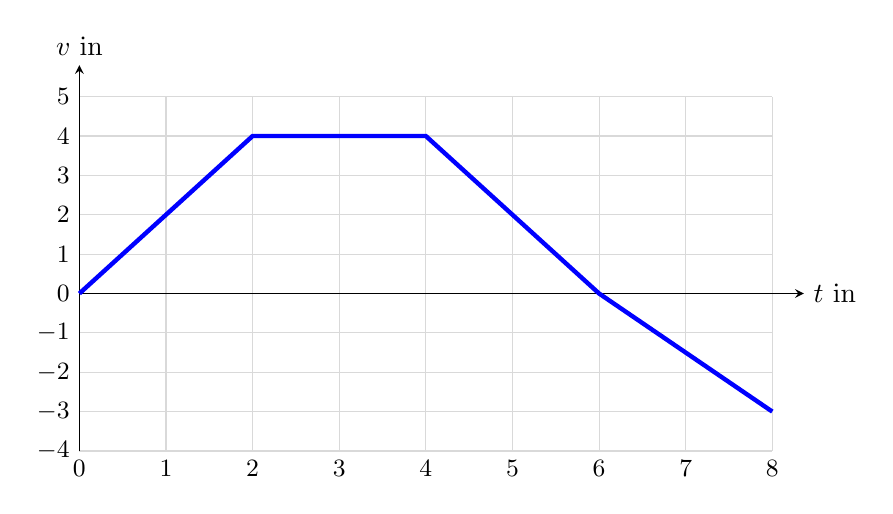
\begin{tikzpicture}[>=stealth, x=1.1cm, y=0.5cm]
 \draw[gray!30] (0,-4) grid[xstep=1, ystep=1] (8,5);
 \draw[->] (0,0) -- (8.364,0) node[right] {$t$ in \si{\second}};
 \draw[->] (0,-4) -- (0,5.8) node[above] {$v$ in \si{\meter\per\second}};
 \foreach \tk in {0,1,2,3,4,5,6,7,8} \node[below] at (\tk,-4) {\small $\tk$};
 \foreach \yk in {-4,-3,-2,-1,0,1,2,3,4,5} \node[left] at (0,\yk) {\small $\yk$};
 \draw[ultra thick, blue] (0,0) -- (2,4) -- (4,4) -- (6,0) -- (8,-3);
\end{tikzpicture}
\end{center}
\begin{abcliste}
\abc Wann ist der Körper am weitesten vom Startpunkt entfernt, und wie weit?
\abc Wie gross ist seine Ortsänderung von \SI{0}{\second} bis \tEndO?
\abc Welche Strecke legt er in dieser Zeit insgesamt zurück?
\end{abcliste}
